\chapter{Genoomstabiliteit: DNA-schade, herstel en recombinatie}\label{ch:b3:dna-repair}

Een middag op het strand brengt zo'n honderdduizend chemische \omterm{def:b3:dna-repair:lesions}{laesies}
aan in het DNA van elke huidcel die aan de zon is blootgesteld:
naburige thymines door ultraviolet licht tot dimeren aaneengesmeed,
basen geoxideerd, strengen ingeknipt. Zelfs zonder een sprankje zon
slaat het warme water van de cel elke dag ongeveer tienduizend purines
van hun suikers af en maakt het van honderden cytosines uracil. Toch
bedraagt de mutatiesnelheid van een menselijke cel ongeveer één
verandering per tien miljard basenparen per deling --- in een genoom
van zes miljard minder dan één nieuwe mutatie per deling. Het gat
tussen de schade die een genoom oploopt en de schade die het houdt
wordt gedicht door herstel: een tiental enzymsystemen die de dubbele
helix patrouilleren, herkennen wat er niet hoort te zijn, het
uitknippen en het vanaf de onbeschadigde streng weer opbouwen, en die,
wanneer beide strengen gebroken zijn, ze weer aaneenvoegen of het
ontbrekende stuk van een zusterchromatide kopiëren. De kinderen die
een van deze systemen missen --- die bij de eerste aanraking van
zonlicht verbranden, of die in hun dertiger jaren darmkanker krijgen
--- laten zien wat de systemen waard zijn. Dit hoofdstuk gaat over de
schade, de herstelroutes, de recombinatiemachinerie die de ergste
breuken herstelt en die de meiose te leen neemt, en over het besluit
van de cel om, wanneer het herstel faalt, met delen te stoppen of te
sterven.

\section{Wat er misgaat met DNA}

\begin{definition}[DNA-laesies]\label{def:b3:dna-repair:lesions}
\index{DNA-laesie}\index{depurinering}\index{deaminering}\index{pyrimidinedimeer}\index{dubbelstrengsbreuk}\index{8-oxoguanine}
Een \emph{laesie} is elke chemische verandering van DNA weg van de vier
normale basen, correct gepaard op een intacte ruggengraat. Spontane
laesies ontstaan uit de chemie van water en zuurstof:
\emph{depurinering}, hydrolyse van de binding tussen een purine en
zijn suiker, die een abasische plaats achterlaat (ongeveer $10^{4}$
per cel per dag); \emph{deaminering}, die van cytosine uracil maakt,
van 5-methylcytosine thymine en van adenine hypoxanthine (enkele
honderden per dag); \emph{oxidatie} door reactieve zuurstofsoorten,
vooral tot \emph{8-oxoguanine}, dat even gemakkelijk met adenine als
met cytosine paart; en \emph{replicatiefouten}, een verkeerd ingebouwde
of verschoven base. Laesies uit het milieu zijn onder meer de
\emph{cyclobutaanpyrimidinedimeer} en het 6-4-fotoproduct die
ultraviolet licht tussen twee naburige pyrimidines maakt;
gealkyleerde basen door alkylerende stoffen (O$^{6}$-methylguanine
paart met thymine); volumineuze adducten van aromatische
koolwaterstoffen en aflatoxine; dwarsverbindingen tussen de strengen
door cisplatine en stikstofmosterd; en de enkelstrengs- en
\emph{dubbelstrengsbreuken} die ioniserende straling maakt, ongeveer
\num{1000} enkelstrengs- en \numrange{30}{40} dubbelstrengsbreuken per
cel per gray.
\end{definition}

\begin{proposition}[De getrouwheidsladder]\label{prop:b3:dna-repair:fidelity}
\index{getrouwheid}\index{proeflezen}\index{mismatchherstel}
De replicatie haalt haar foutenpercentage van ongeveer $10^{-10}$ per
basenpaar in drie vermenigvuldigende stappen. De baseselectie door het
polymerase, op geometrie en waterstofbruggen, vergist zich ongeveer
eens per $10^{5}$; het \emph{proeflezen} door het 3$'\to$5$'$-exonuclease
van het polymerase, dat een verkeerd gepaarde eindbase verwijdert
voordat er wordt verlengd, haalt daar \qty{99}{\%} van weg; het
\emph{\omterm{prop:b3:dna-repair:fidelity}{mismatchherstel}}, dat achter de vork op de nieuw gemaakte streng
werkt, haalt \qty{99.9}{\%} van de rest weg. Het product
$10^{-5}\times 10^{-2}\times 10^{-3} = 10^{-10}$ is de waargenomen
snelheid, en een defect in een van beide correctiestappen verhoogt haar
honderd- of duizendvoudig: zulke cellen zijn \emph{mutatoren}.
\end{proposition}

\begin{example}[Laesies tegenover mutaties]\label{ex:b3:dna-repair:numbers}
Een menselijke cel van $6.4\times 10^{9}$ basenparen die zich eens per
dag deelt stapelt in de orde van $10^{4}$--$10^{5}$ \omterm{def:b3:dna-repair:lesions}{laesies} per dag op
en ongeveer $6.4\times 10^{9}\times 10^{-10} \approx 0.6$ nieuwe
mutaties per deling: minder dan één \omterm{def:b3:dna-repair:lesions}{laesie} op tienduizend overleeft om
een blijvende verandering te worden. De rest wordt hersteld voordat de
replicatie ze afleest, en wat de selectie heeft geminimaliseerd is de
kans dat een \omterm{def:b3:dna-repair:lesions}{laesie} tot mutatie uitgroeit, niet de hoeveelheid schade.
Dezelfde rekensom laat zien waarom het aantal mutaties in een tumor of
in het zaad van een oudere vader delingen telt: de mutaties die een cel
draagt zijn in eerste benadering het aantal delingen dat zij heeft
doorgemaakt maal de fout per deling.
\end{example}

\section{Herstel van één beschadigde streng}

\begin{definition}[Excisieherstel]\label{def:b3:dna-repair:excision}
\index{base-excisieherstel}\index{nucleotide-excisieherstel}\index{glycosylase}\index{xeroderma pigmentosum}
De meeste \omterm{def:b3:dna-repair:lesions}{laesies} treffen één streng en worden hersteld door het
beschadigde stuk uit te knippen en de andere streng te kopiëren. Het
\emph{base-excisieherstel} (BER) doet kleine, niet vervormende
\omterm{def:b3:dna-repair:lesions}{laesies}: een \emph{DNA-glycosylase} dat specifiek is voor één soort
verkeerde base (uracil-DNA-glycosylase, 8-oxoG-glycosylase en
verscheidene andere) klapt de base uit de helix en knipt haar van haar
suiker; een AP-endonuclease knipt de ruggengraat in bij de abasische
plaats; een polymerase (Pol~$\beta$) verwijdert de suiker en zet één
nucleotide in; een ligase sluit. Het \emph{nucleotide-excisieherstel}
(NER) doet volumineuze \omterm{def:b3:dna-repair:lesions}{laesies} die de helix vervormen ---
pyrimidinedimeren, chemische adducten --- zonder de chemie van de
\omterm{def:b3:dna-repair:lesions}{laesie} zelf te herkennen: de vervorming wordt opgemerkt (door XPC dat
het genoom afspeurt, of door een gestrand RNA-polymerase in de aan
transcriptie gekoppelde tak), de helix wordt geopend door de
helicase-subeenheden van TFIIH, de schade wordt geverifieerd (XPA),
twee endonucleasen (XPF, XPG) knippen de beschadigde streng
\numrange{24}{32} nucleotiden uit elkaar, het oligonucleotide komt
vrij, en polymerase en ligase vullen het gat. Verlies van een van de
zeven XP-eiwitten veroorzaakt \emph{xeroderma pigmentosum}: extreme
gevoeligheid voor zonlicht, sproeten, en een duizendvoudig verhoogde
kans op huidkanker.
\end{definition}

\begin{proof}[Bewijsmateriaal]
Cleaver (1968) kweekte huidfibroblasten van patiënten met \omterm{def:b3:dna-repair:excision}{xeroderma
pigmentosum}, bestraalde ze met ultraviolet licht en gaf ze buiten de
S-fase radioactief thymidine. Normale cellen bouwden het merkstof op
vele kleine plaatsen in --- de ``ongeplande DNA-synthese'' van de
herstelplekken --- terwijl de cellen van de patiënten er vrijwel niets
van inbouwden en stierven bij doses die normale cellen overleefden: de
ziekte is een onvermogen om de dimeren uit te snijden. Het versmelten
van cellen van twee patiënten herstelde in de hybride vaak het
herstel, waarbij elke cel leverde wat de andere miste; met die toets
werden de patiënten in complementatiegroepen A tot G ingedeeld, één
per gen van de route, jaren voordat de genen werden gekloneerd.
\end{proof}

\begin{omfigure}
\begin{tikzpicture}[every node/.style={font=\scriptsize}, >=stealth]
  % BER column
  \node[font=\small\bfseries] at (2.0,3.2) {Base-excisieherstel};
  \foreach \y/\txt in {2.6/{beschadigde base (U, 8-oxoG)}, 1.5/{glycosylase haalt de base weg}, 0.4/{AP-endonuclease knipt in}, -0.7/{Pol $\beta$ vult één nucleotide, ligase sluit}} {
    \draw[very thick, omDef] (0.2,\y) -- (3.8,\y); \draw[very thick, omDef] (0.2,\y-0.25) -- (3.8,\y-0.25);
    \node[right, align=left] at (0.2,\y-0.6) {\txt};
  }
  \fill[omThm] (2.0,2.6) circle (0.1);
  \draw[omThm, thick] (1.9,1.5) -- (2.1,1.5);
  \draw[white, very thick] (1.9,0.4) -- (2.1,0.4);
  \fill[omMeth!80!black] (2.0,-0.7) circle (0.1);
  % NER column
  \node[font=\small\bfseries] at (8.0,3.2) {Nucleotide-excisieherstel};
  \foreach \y/\txt in {2.6/{volumineuze laesie vervormt de helix; XPC bindt}, 1.5/{TFIIH opent de helix, XPA verifieert}, 0.4/{XPF en XPG knippen 24--32 nt uit elkaar}, -0.7/{polymerase vult het gat, ligase sluit}} {
    \draw[very thick, omDef] (6.2,\y) -- (9.8,\y); \draw[very thick, omDef] (6.2,\y-0.25) -- (9.8,\y-0.25);
    \node[right, align=left] at (6.2,\y-0.6) {\txt};
  }
  \draw[omThm, very thick] (7.8,2.6) -- (8.2,2.6) -- (8.2,2.75) -- (7.8,2.75) -- cycle;
  \draw[omDef, very thick] (7.2,1.5) .. controls (7.6,1.85) and (8.4,1.85) .. (8.8,1.5); \draw[omThm, very thick] (7.85,1.72) -- (8.15,1.72);
  \draw[very thick, white] (7.0,0.4) -- (9.0,0.4); \draw[omThm, thick, ->] (7.0,0.7) -- (7.0,0.48); \draw[omThm, thick, ->] (9.0,0.7) -- (9.0,0.48);
  \draw[very thick, omMeth!80!black] (7.0,-0.7) -- (9.0,-0.7);
\end{tikzpicture}

{\small Twee excisieroutes. Base-excisie (links) herkent met een eigen
\omterm{def:b3:dna-repair:excision}{glycosylase} één bepaalde verkeerde base en vervangt één nucleotide.
Nucleotide-excisie (rechts) herkent de vervorming die elke
volumineuze \omterm{def:b3:dna-repair:lesions}{laesie} veroorzaakt, knipt de streng aan weerszijden door
en vervangt een plek van zo'n dertig nucleotiden (groen).}
\end{omfigure}

\begin{definition}[Mismatchherstel]\label{def:b3:dna-repair:mmr}
\index{mismatchherstel!strengonderscheiding}\index{syndroom van Lynch}\index{microsatellietinstabiliteit}
Het \emph{\omterm{prop:b3:dna-repair:fidelity}{mismatchherstel}} (MMR) corrigeert de verkeerde paringen en
kleine insertie-deletielussen die aan het proeflezen ontsnappen. Het
MutS-eiwit (MSH2--MSH6 bij de mens) herkent de vervorming van een
mismatch en geeft, met MutL (MLH1--PMS2), een exonuclease toestemming
om de nieuw gemaakte streng vanaf een nabije inknip tot voorbij de
mismatch af te breken; het gat wordt door het polymerase weer gevuld.
De moeilijkheid is de \emph{strengonderscheiding}: een mismatch heeft
twee basen en maar één ervan is fout. Bij \emph{Escherichia coli}
wordt de nieuwe streng herkend doordat zij bij de GATC-plaatsen nog
niet is gemethyleerd, wat het Dam-methylase enkele minuten na de
synthese doet; MutH knipt de ongemethyleerde streng in. Bij eukaryoten
wordt de nieuwe streng herkend aan de inknipjes tussen de
Okazaki-fragmenten en aan het vrije 3$'$-uiteinde van de leidende
streng. Verlies van MMR verhoogt de mutatiesnelheid honderd- tot
duizendvoudig, het duidelijkst bij \emph{microsatellieten} --- reeksen
van een korte herhaling waar het polymerase uitglijdt --- waarvan de
lengtes van cel tot cel verschillen: \emph{microsatellietinstabiliteit}.
Erfelijk verlies van één MMR-allel is het \emph{syndroom van Lynch},
met darmkanker bij zo'n \qty{70}{\%} van de dragers, vaak vóór hun
vijftigste.
\end{definition}

\begin{omfigure}
\begin{tikzpicture}[every node/.style={font=\scriptsize}, >=stealth]
  \draw[very thick, omDef] (0,1.2) -- (9,1.2); \node[left] at (-0.1,1.2) {matrijsstreng};
  \draw[very thick, gray] (0,0.6) -- (9,0.6); \node[left] at (-0.1,0.6) {nieuwe streng};
  % methyl groups on template at GATC
  \foreach \x in {1.5,7.5} { \fill[omMeth!80!black] (\x,1.35) circle (0.1); \node[above] at (\x,1.45) {CH$_3$ op GATC}; }
  \foreach \x in {1.5,7.5} { \draw[omMeth!80!black] (\x,0.45) circle (0.1); }
  \node[below] at (7.5,0.32) {nog niet gemethyleerd};
  % mismatch
  \draw[omThm, very thick] (4.5,1.05) -- (4.5,0.75); \node[omThm, right] at (4.6,0.9) {mismatch};
  \draw[thick, fill=omExo!35] (4.5,1.9) ellipse (1.0 and 0.3); \node at (4.5,1.9) {MutS/MutL};
  \draw[->, thick] (4.5,1.65) -- (4.5,1.3);
  % MutH nick on new strand at unmethylated GATC
  \draw[omThm, thick, ->] (1.5,-0.55) -- (1.5,0.42); \node[omThm, below] at (1.5,-0.55) {MutH knipt de ongemethyleerde streng in};
  % excision arrow
  \draw[->, very thick, omProp] (1.7,-0.1) -- (5.0,-0.1); \node[omProp, below] at (3.95,-0.15) {exonuclease breekt af tot voorbij de mismatch};
  \node[right] at (5.4,-0.8) {daarna vult Pol III het gat, ligase sluit};
\end{tikzpicture}

{\small Strengonderscheiding bij het bacteriële \omterm{prop:b3:dna-repair:fidelity}{mismatchherstel}. De
matrijsstreng draagt methylgroepen op haar GATC-plaatsen; de nieuwe
streng nog niet, en MutH knipt haar daar in. De verkeerde base wordt
dus altijd van de nieuwe streng verwijderd.}
\end{omfigure}

\begin{method}[Een herstelziekte in genen indelen]\label{met:b3:dna-repair:complementation}
\index{complementatietest}
Om te vinden hoeveel genen bij een recessief fenotype betrokken zijn,
nog voordat er één gen bekend is: (1) neem cellijnen van niet-verwante
patiënten, elk mutant in een of ander gen van de route; (2) versmelt
paren van lijnen tot hybride cellen; (3) toets de hybride op de functie
(hier de ongeplande DNA-synthese na ultraviolet licht); (4) is de
hybride hersteld, dan dragen de twee patiënten mutaties in
\emph{verschillende} genen (elk levert het eiwit dat de ander mist: zij
\emph{complementeren}); zo niet, dan in hetzelfde gen; (5) deel de
patiënten in complementatiegroepen in --- één per gen. Het aantal
groepen is een ondergrens voor het aantal genen.
\end{method}

\section{Herstel van een gebroken chromosoom}

\begin{definition}[Herstel van dubbelstrengsbreuken]\label{def:b3:dna-repair:dsb}
\index{niet-homologe eindverbinding}\index{homologe recombinatie}\index{Rad51}\index{Holliday-junctie}\index{BRCA}
Een \emph{\omterm{def:b3:dna-repair:lesions}{dubbelstrengsbreuk}} doorsnijdt het chromosoom en laat geen
intacte streng over om te kopiëren. Twee routes herstellen haar. De
\emph{niet-homologe eindverbinding} (NHEJ): de Ku70--Ku80-ring bindt
elk uiteinde, trekt het kinase DNA-PKcs aan, nucleasen snoeien de
overhangen bij, en ligase IV voegt de uiteinden samen; zij werkt in elk
stadium van de cyclus en binnen minuten, maar verliest of voegt enkele
nucleotiden toe bij de las en kan de verkeerde uiteinden samenvoegen.
De \emph{homologe recombinatie} (HR): het MRN-complex en nucleasen
snoeien de 5$'$-strengen weg en laten lange enkelstrengs
3$'$-staarten achter, die door RPA en daarna, met hulp van BRCA2, door
het recombinase \emph{Rad51} worden bekleed; het Rad51-filament zoekt
een homologe duplex --- de zusterchromatide, in S en G2 --- dringt die
binnen, en het binnendringende 3$'$-uiteinde start de synthese op de
intacte kopie. De verbonden moleculen kunnen na een korte synthese
worden losgemaakt (het meeste mitotische herstel, zonder uitwisseling
van flankerend DNA) of uitgroeien tot twee vierarmige
\emph{Holliday-juncties}, waarvan de oplossing door endonucleasen
ofwel een crossover ofwel een niet-crossoverproduct geeft. HR is
nauwkeurig omdat zij een zuster kopieert, maar is alleen beschikbaar
wanneer er een zuster is.
\end{definition}

\begin{omfigure}
\begin{tikzpicture}[every node/.style={font=\scriptsize}, >=stealth]
  % break
  \draw[very thick, omDef] (0,3.2) -- (2.3,3.2); \draw[very thick, omDef] (2.7,3.2) -- (5,3.2);
  \draw[very thick, omDef] (0,3.0) -- (2.3,3.0); \draw[very thick, omDef] (2.7,3.0) -- (5,3.0);
  \node[above] at (2.5,3.3) {dubbelstrengsbreuk};
  % NHEJ left
  \draw[->, thick] (1.2,2.8) -- (-0.5,2.0); \node[left, align=right] at (-0.6,2.4) {elke fase,\\minuten};
  \node[font=\small\bfseries] at (-1.6,1.55) {NHEJ};
  \draw[thick, fill=omExo!35] (-2.6,0.9) ellipse (0.3 and 0.2); \draw[thick, fill=omExo!35] (-0.8,0.9) ellipse (0.3 and 0.2);
  \draw[very thick, omDef] (-3.4,0.9) -- (-2.9,0.9); \draw[very thick, omDef] (-0.5,0.9) -- (0.0,0.9);
  \node[below] at (-1.7,0.7) {Ku bindt beide uiteinden, bijsnoeien};
  \draw[->, thick] (-1.7,0.3) -- (-1.7,-0.1);
  \draw[very thick, omDef] (-3.4,-0.4) -- (0.0,-0.4); \draw[omThm, very thick] (-1.85,-0.4) -- (-1.55,-0.4);
  \node[below, align=center] at (-1.7,-0.55) {ligase IV voegt samen:\\enkele nucleotiden weg of erbij};
  % HR right
  \draw[->, thick] (3.8,2.8) -- (5.5,2.0); \node[right, align=left] at (5.6,2.4) {S/G2, een zuster\\aanwezig; uren};
  \node[font=\small\bfseries] at (6.8,1.55) {HR};
  % resected ends
  \draw[very thick, omDef] (4.6,0.9) -- (6.2,0.9); \draw[very thick, omDef] (7.4,0.9) -- (9.0,0.9);
  \draw[very thick, omDef] (4.6,0.7) -- (5.6,0.7); \draw[very thick, omDef] (8.0,0.7) -- (9.0,0.7);
  \foreach \x in {5.7,5.9,6.1} \fill[omProp] (\x,0.9) circle (0.07);
  \node[below] at (6.8,0.55) {5$'$-wegsnoeien; Rad51 bekleedt de 3$'$-staarten};
  \draw[->, thick] (6.8,0.15) -- (6.8,-0.25);
  % strand invasion of sister
  \draw[very thick, omMeth!70!black] (4.6,-0.9) -- (9.0,-0.9); \draw[very thick, omMeth!70!black] (4.6,-1.1) -- (9.0,-1.1);
  \draw[very thick, omDef] (4.6,-0.5) -- (5.8,-0.5) .. controls (6.2,-0.5) and (6.3,-0.9) .. (6.6,-0.9) -- (7.6,-0.9);
  \draw[->, omDef, thick] (7.6,-0.9) -- (8.1,-0.9);
  \node[below, align=center] at (6.8,-1.2) {binnendringen van de zuster (groen), synthese op de intacte kopie,\\daarna losmaken (geen crossover) of Holliday-juncties};
\end{tikzpicture}

{\small De twee lotgevallen van een \omterm{def:b3:dna-repair:lesions}{dubbelstrengsbreuk}. Links: het
samenvoegen van uiteinden, snel en altijd beschikbaar, ten koste van
een kleine verandering bij de las. Rechts: de \omterm{def:b3:dna-repair:dsb}{homologe recombinatie},
die de uiteinden wegsnoeit, met een Rad51-filament de zusterchromatide
binnendringt en kopieert wat verloren ging.}
\end{omfigure}

\begin{theorem}[Schadelast, herstelsnelheid en de vork]\label{thm:b3:dna-repair:load}
\index{restschade}\index{concurrerende routes}
Laat \omterm{def:b3:dna-repair:lesions}{laesies} van één soort met constante snelheid $D$ per cel per uur
ontstaan en met eerste-ordeherstel met snelheidsconstante $k$ worden
verwijderd (halveringstijd $t_{1/2} = \ln 2/k$). Het aantal \omterm{def:b3:dna-repair:lesions}{laesies}
$L(t)$ voldoet aan $\mathrm{d}L/\mathrm{d}t = D - kL$, zodat in
evenwicht
\[
L^{*} = \frac{D}{k},
\]
en een puls van $N$ \omterm{def:b3:dna-repair:lesions}{laesies} die op $t = 0$ wordt toegediend laat
$N e^{-kT}$ \omterm{def:b3:dna-repair:lesions}{laesies} over wanneer een replicatievork op tijdstip $T$
aankomt. Concurreren twee routes om dezelfde \omterm{def:b3:dna-repair:lesions}{laesie} met
snelheidsconstanten $k_{1}$ en $k_{2}$, dan wordt elke \omterm{def:b3:dna-repair:lesions}{laesie} door de
eerste hersteld met kans $k_{1}/(k_{1} +
k_{2})$ en is de totale halveringstijd $\ln 2/(k_{1} + k_{2})$. Het
aantal \omterm{def:b3:dna-repair:lesions}{laesies} dat de vork bereikt is poissonverdeeld met gemiddelde
$N e^{-kT}$, dus is de kans dat er geen enkele aankomt $\exp(-N e^{-kT})$.
\end{theorem}
\begin{proof}
Het evenwicht ligt waar $D = kL$. Voor de puls is $D = 0$ en
integreert de vergelijking tot $L = N e^{-kt}$. Met twee routes is de
verliessnelheid $(k_{1} + k_{2})L$; in elk kort tijdsinterval wordt een
gegeven \omterm{def:b3:dna-repair:lesions}{laesie} door route~1 verwijderd met kans $k_{1}\,\mathrm{d}t$ en
door route~2 met $k_{2}\,\mathrm{d}t$, dus is de voorwaardelijke kans
dat haar verwijdering, wanneer die plaatsvindt, door route~1 gebeurt
$k_{1}/(k_{1} +
k_{2})$. Onafhankelijke \omterm{def:b3:dna-repair:lesions}{laesies} die elk met kans $e^{-kT}$ overleven
geven een binomiale telling, poisson in de limiet van veel \omterm{def:b3:dna-repair:lesions}{laesies} en
kleine overleving, en de poissonkans op nul is $e^{-\text{gemiddelde}}$.
\end{proof}

\begin{example}[Waarom xeroderma een ziekte van de vork is]\label{ex:b3:dna-repair:xp}
Een dosis zon laat $N = 10^{5}$ pyrimidinedimeren in een keratinocyt
achter. Met een halveringstijd van het \omterm{def:b3:dna-repair:excision}{nucleotide-excisieherstel} van
\qty{2}{h} ($k =
\qty{0.35}{h^{-1}}$) en een vork die na \qty{8}{h} aankomt, zijn er
$N e^{-kT} =
10^{5}\times e^{-2.8} \approx 6000$ dimeren over om te worden
gekopieerd; met het vrijwel afwezige herstel van een XP-cel ($k \approx
\qty{0.01}{h^{-1}}$) zijn dat er \num{92000}. Elke dimeer die de vork
tegenkomt wordt overbrugd door \omterm{def:b3:dna-repair:tls}{translesiesynthese} (hieronder), die
foutgevoelig is: de mutatielast per deling van de patiënt is vijftien
keer de normale, en de huidkankers volgen al in de kindertijd. De
remedie die werkt is $N$ klein houden --- ultraviolet licht volledig
mijden.
\end{example}

\begin{omfigure}
\begin{tikzpicture}
\begin{axis}[
  width=0.7\linewidth, height=5.6cm,
  axis x line=bottom, axis y line=left,
  xmin=0, xmax=12, ymin=100, ymax=200000, ymode=log,
  xlabel={uren na blootstelling}, ylabel={dimeren per cel},
  xlabel style={font=\small, at={(axis description cs:0.5,-0.12)}, anchor=north},
  ylabel style={font=\small},
  tick label style={font=\small}, xtick={0,2,4,6,8,10,12},
  clip=false,
]
\addplot[very thick, omDef, domain=0:12, samples=40] {100000*exp(-0.35*x)};
\addplot[very thick, omThm, domain=0:12, samples=40] {100000*exp(-0.01*x)};
\addplot[dashed, gray] coordinates {(8,100) (8,200000)};
\node[font=\scriptsize, anchor=south east, gray] at (axis cs:8,110) {vork komt aan};
\node[font=\scriptsize, omDef, anchor=north east] at (axis cs:11.5,18000) {normaal, $t_{1/2} = \qty{2}{h}$};
\node[font=\scriptsize, omThm, anchor=south west] at (axis cs:2,105000) {xeroderma pigmentosum};
\fill[omDef] (axis cs:8,6070) circle (2pt); \node[font=\scriptsize, omDef, anchor=west] at (axis cs:8.3,6070) {\num{6000}};
\fill[omThm] (axis cs:8,92300) circle (2pt); \node[font=\scriptsize, omThm, anchor=north west] at (axis cs:8.3,80000) {\num{92000}};
\end{axis}
\end{tikzpicture}

{\small Overgebleven dimeren na een puls van $10^{5}$, op een
logaritmische schaal, voor een normale cel en een cel zonder
\omterm{def:b3:dna-repair:excision}{nucleotide-excisieherstel}. De vork bij \qty{8}{h} treft in de cel van
de patiënt vijftien keer meer \omterm{def:b3:dna-repair:lesions}{laesies} aan.}
\end{omfigure}

\begin{proof}[Bewijsmateriaal]
Holliday (1964) stelde de vierarmige junctie voor om een raadsel uit de
schimmelgenetica te verklaren: bij een kruising vertoonde een tetrade
van sporen soms een splitsing $3{:}1$ in plaats van de mendeliaanse
$2{:}2$ van een merker, altijd bij merkers vlak bij een crossover. Zijn
model --- de uitwisseling van enkele strengen tussen twee homologe
duplexen, waarbij een heteroduplex ontstaat die het \omterm{prop:b3:dna-repair:fidelity}{mismatchherstel}
daarna in de ene of de andere richting ``corrigeert''
(\emph{genconversie}) --- verklaarde zowel de vreemde verhoudingen als
hun samengaan met crossing-over. De junctie zelf werd later in de
elektronenmicroscoop gezien in recombinerende plasmiden en in de
structuur van het resolvase RuvC dat eraan gebonden is.
\end{proof}

\section{Tolerantie, alarm en het besluit om te stoppen}

\begin{definition}[Translesiesynthese]\label{def:b3:dna-repair:tls}
\index{translesiesynthese}\index{polymerase eta}
Wanneer een vork een \omterm{def:b3:dna-repair:lesions}{laesie} tegenkomt die niet is hersteld, strandt het
replicatieve polymerase. De \emph{translesiesynthese} (TLS) roept een
gespecialiseerd polymerase met een ruimere actieve plaats en zonder
proeflezen erbij --- Pol~$\eta$ voor pyrimidinedimeren, Pol~$\iota$,
$\kappa$, $\zeta$ en Rev1 voor andere \omterm{def:b3:dna-repair:lesions}{laesies} --- dat enkele
nucleotiden tegenover de \omterm{def:b3:dna-repair:lesions}{laesie} zet en daarna opzij gaat. Pol~$\eta$
zet twee adenines tegenover een thyminedimeer, wat meestal juist is;
de andere zitten er vaak naast. TLS ruilt nauwkeurigheid in voor het
voortbestaan van de vork, en is de bron van de meeste mutaties die
ultraviolet licht veroorzaakt. De variantvorm van \omterm{def:b3:dna-repair:excision}{xeroderma
pigmentosum} (XP-V) heeft een intact excisieherstel en mist
Pol~$\eta$: de dimeren die aan de excisie ontsnappen worden door de
foutgevoeliger polymerasen overbrugd, en de kankers volgen.
\end{definition}

\begin{proposition}[De bacteriële SOS-respons]\label{prop:b3:dna-repair:sos}
\index{SOS-respons}\index{RecA}\index{LexA}
Bij \emph{E.~coli} wordt het recombinase RecA, gebonden aan het
enkelstrengs DNA dat zich bij gestrande vorken en weggesnoeide breuken
ophoopt, een co-protease dat de repressor LexA ertoe brengt zichzelf te
knippen. LexA onderdrukt zo'n veertig genen; naarmate hij wegvalt gaan
ze aan in de volgorde van de affiniteit van hun operatoren: eerst de
excisieherstelgenen \emph{uvrA} en \emph{uvrB}, dan \emph{recA} zelf en
de celdelingsremmer \emph{sulA} (de cellen stoppen met delen en groeien
uit tot filamenten), en als laatste de foutgevoelige polymerasen
Pol~IV en Pol~V, die \omterm{def:b3:dna-repair:lesions}{laesies} overbruggen ten koste van mutaties. De
getrapte respons probeert eerst nauwkeurig herstel en pas mutagene
tolerantie wanneer de schade aanhoudt; de mutaties die zij opwekt zijn
het ruwe materiaal waarop antibioticaresistentie tijdens een
behandeling evolueert.
\end{proposition}

\begin{omfigure}
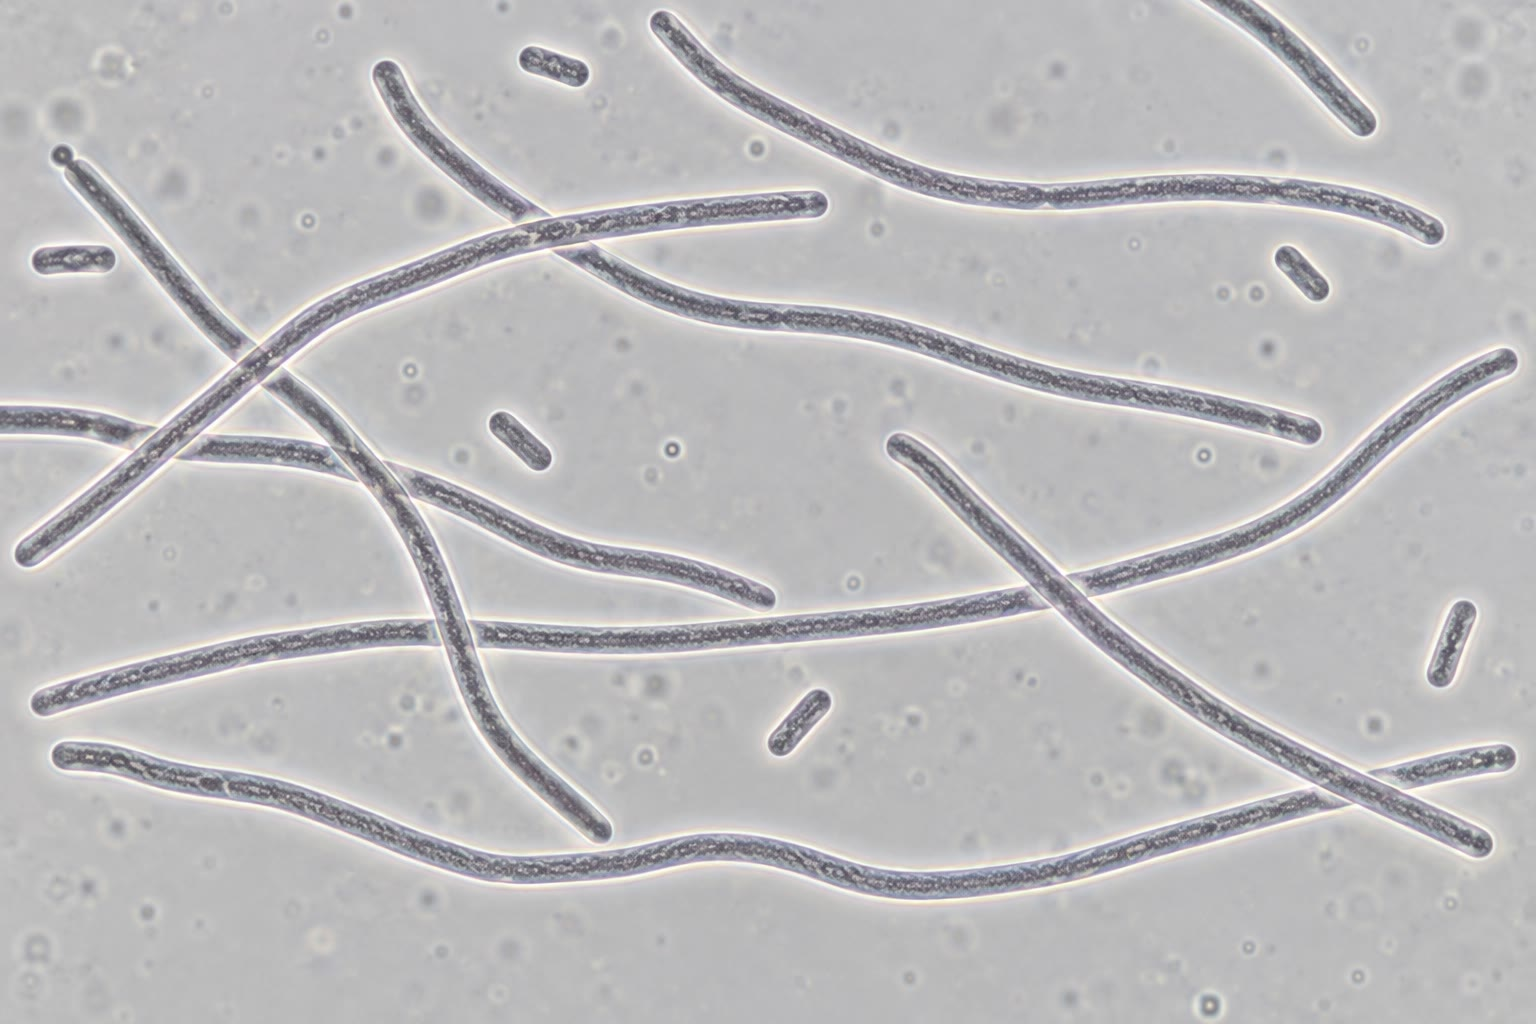
\includegraphics[width=0.46\linewidth]{images/book5/ai/b5-03-sos-filaments.jpg}\hspace{0.04\linewidth}
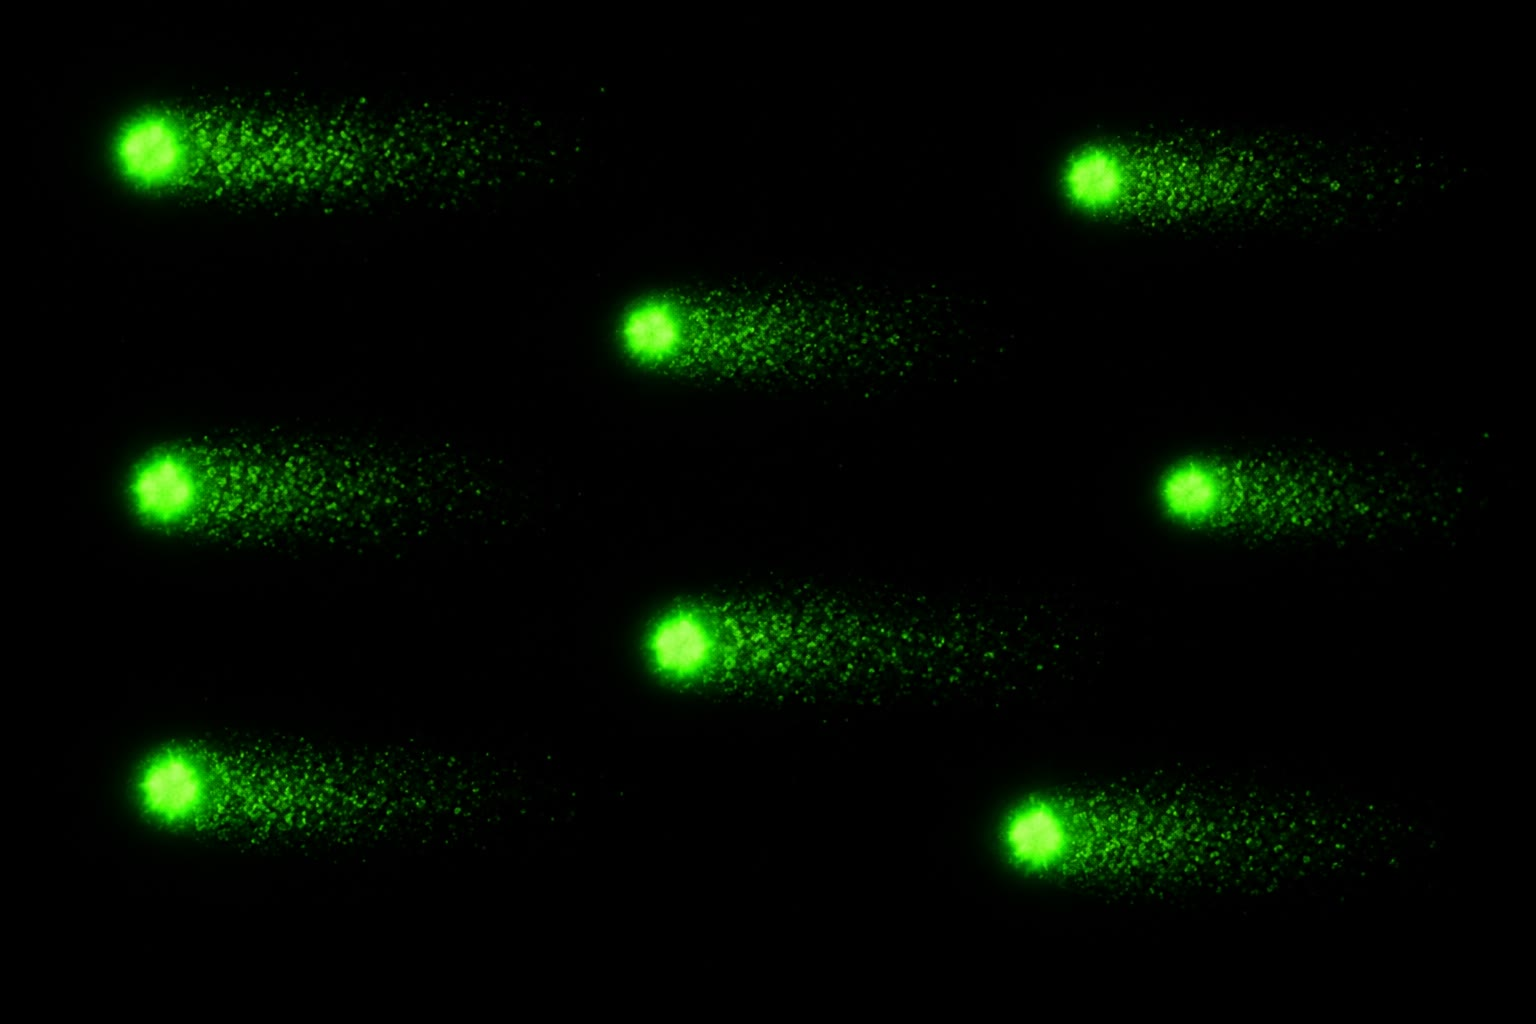
\includegraphics[width=0.46\linewidth]{images/book5/ai/b5-03-comet-assay.jpg}

{\small Links: \emph{E.~coli} na bestraling met ultraviolet licht,
uitgegroeid tot lange filamenten omdat de \omterm{prop:b3:dna-repair:sos}{SOS-respons} de celdeling
heeft geblokkeerd terwijl het DNA wordt hersteld. Rechts: een
comettest --- afzonderlijke cellen ingebed in een gel en
geëlektroforeerd; gefragmenteerd DNA stroomt de kern uit in een staart
waarvan de lengte het aantal breuken meet.}
\end{omfigure}

\begin{definition}[De DNA-schaderespons]\label{def:b3:dna-repair:ddr}
\index{DNA-schaderespons}\index{ATM}\index{controlepunt}\index{p53}\index{gamma-H2AX}
Eukaryoten geven schade door via twee kinasen: \emph{ATM}, dat door het
MRN-complex naar \omterm{def:b3:dna-repair:lesions}{dubbelstrengsbreuken} wordt gebracht, en \emph{ATR},
dat naar het enkelstrengs DNA van gestrande vorken wordt gebracht. Zij
fosforyleren honderden doelwitten. Binnen enkele minuten wordt het
\omterm{def:b3:chromatin-epigenetics:nucleosome}{histon} H2AX gefosforyleerd (\emph{$\gamma$-H2AX}) over megabasen rond
elke breuk, wat een focus vormt die hersteleiwitten aantrekt en onder
de microscoop kan worden geteld, één focus per breuk. De kinasen Chk1
en Chk2 leggen de celcyclus stil --- de \emph{controlepunten} van
\cref{ch:b3:cell-cycle-apoptosis} --- door de fosfatasen te
inactiveren die de intrede in S of M zouden aandrijven; en de
transcriptiefactor \emph{p53}, gestabiliseerd door fosforylering,
induceert de remmer p21 van cycline-afhankelijke kinasen (een duurzame
stilstand in G1), herstelgenen en, als de schade zwaar is of aanhoudt,
de apoptosegenen die de cel doden. De respons koopt tijd voor herstel,
en wanneer het herstel faalt ruimt zij de cel op in plaats van haar met
een gebroken genoom te laten delen.
\end{definition}

\begin{omfigure}
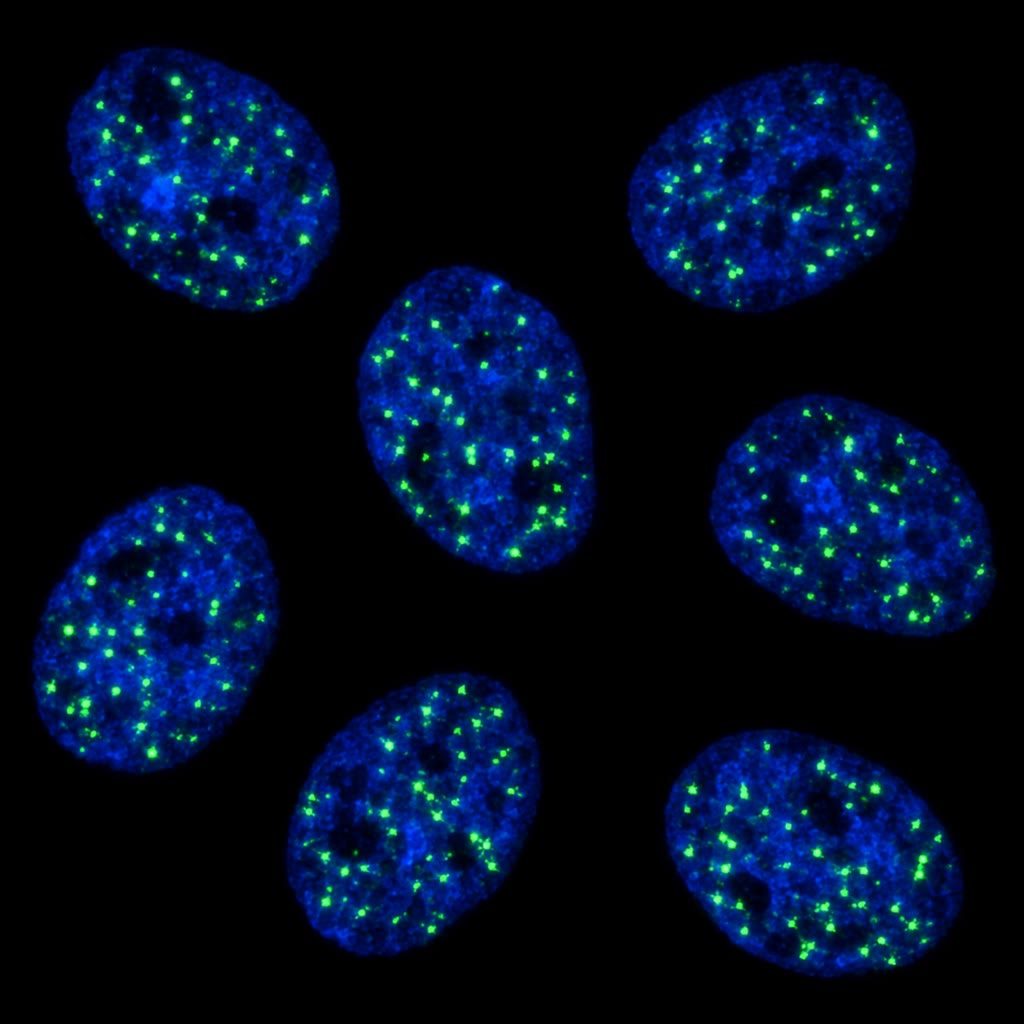
\includegraphics[width=0.4\linewidth]{images/book5/ai/b5-03-gamma-foci.jpg}

{\small $\gamma$-H2AX-foci (groen) in kernen (blauw) een uur na
bestraling. Elke focus markeert een \omterm{def:b3:dna-repair:lesions}{dubbelstrengsbreuk}; ze tellen meet
de schade en, in de uren erna, het herstel ervan.}
\end{omfigure}

\begin{example}[Synthetische lethaliteit: BRCA en PARP]\label{ex:b3:dna-repair:parp}
Vrouwen die één defecte kopie van \emph{BRCA1} of \emph{BRCA2} erven
hebben een levenslang risico op borstkanker van \qtyrange{50}{80}{\%};
de tumoren ontstaan in cellen die de tweede kopie hebben verloren en
geen \omterm{def:b3:dna-repair:dsb}{homologe recombinatie} meer kunnen doen. Zulke cellen herstellen
hun \omterm{def:b3:dna-repair:lesions}{dubbelstrengsbreuken} alleen nog met eindverbinding en stapelen
herschikkingen op. Zij verwerven ook een bijzondere zwakte.
Enkelstrengsbreuken, zo'n \num{10000} per dag, worden hersteld langs
een route die het enzym PARP nodig heeft; wordt PARP door een
geneesmiddel geremd, dan blijven enkelstrengsbreuken tot in de S-fase
bestaan, waar een vork er elk in een \omterm{def:b3:dna-repair:lesions}{dubbelstrengsbreuk} met maar één
uiteinde omzet --- alleen door recombinatie te herstellen. Een normale
cel, met één goed \emph{\omterm{def:b3:dna-repair:dsb}{BRCA}}-allel, redt zich; de tumorcel sterft.
Twee defecten, elk op zichzelf onschadelijk, zijn samen dodelijk: het
geneesmiddel doodt door \emph{synthetische lethaliteit}, en spaart de
andere cellen van de patiënt.
\end{example}

\begin{proposition}[Recombinatie als gereedschap]\label{prop:b3:dna-repair:tools}
\index{plaatsspecifieke recombinatie}\index{Cre-lox}
Plaatsspecifieke recombinasen knippen DNA op korte, vastgelegde
sequenties en voegen het weer samen, zonder zoektocht naar homologie of
synthese: het enzym Cre van faag P1 werkt op \emph{loxP}-plaatsen van
\qty{34}{bp}, het gistenzym Flp op \emph{FRT}-plaatsen. Twee plaatsen
in dezelfde richting op één molecuul snijden het DNA ertussen als een
cirkel eruit; in tegengestelde richting draaien zij het om; plaatsen op
twee moleculen wisselen hun flanken uit. Een gen dat door
\emph{loxP}-plaatsen wordt geflankeerd (``gefloxt'') wordt alleen
verwijderd in de cellen waar Cre tot expressie komt, vanaf een promotor
naar keuze van de onderzoeker, of op een tijdstip naar diens keuze
wanneer Cre door een geneesmiddel actief wordt gemaakt: zo wordt een
gen dat voor het embryo onmisbaar is toch in de volwassen lever
bestudeerd, of alleen in een neuron
(\cref{ch:b3:genetic-engineering}). De eigen \omterm{def:b3:dna-repair:dsb}{homologe recombinatie} van
de cel is wat gerichte genmodificatie en CRISPR-gestuurd bewerken te
leen nemen om een gekozen sequentie op een gekozen plaats te schrijven.
\end{proposition}

\begin{remark}[Herstel en veroudering]\label{rem:b3:dna-repair:ageing}
Cellen die niet herstellen stapelen mutaties op, gaan in senescentie of
sterven; de erfelijke herstelgebreken (het syndroom van Werner, een
helicase; het syndroom van Cockayne, het aan transcriptie gekoppelde
herstel; ataxia teleangiëctasia, \omterm{def:b3:dna-repair:ddr}{ATM}) veroorzaken kenmerken van
vroegtijdige veroudering, en het aantal somatische mutaties in normale
weefsels stijgt lineair met de leeftijd, met enkele tientallen mutaties
per cel per jaar. Of opgestapelde schade de gewone veroudering
\emph{veroorzaakt}, dan wel haar alleen vergezelt, is niet beslecht;
dat het herstelvermogen tussen soorten een bepalende factor voor de
levensduur is --- langer levende soorten herstellen meer --- is goed
onderbouwd.
\end{remark}

\section{Opgaven}

\begin{exercise}[$\star$]\label{exo:b3:dna-repair:1}
Deel deze \omterm{def:b3:dna-repair:lesions}{laesies} in als spontaan of uit het milieu en noem voor elk de
herstelroute: een uracil in DNA; een thyminedimeer; een \omterm{def:b3:dna-repair:lesions}{8-oxoguanine};
een G--T-mismatch achter de vork; een \omterm{def:b3:dna-repair:lesions}{dubbelstrengsbreuk} in G1.
\end{exercise}

\begin{exercise}[$\star$]\label{exo:b3:dna-repair:2}
Waarom heeft het \omterm{def:b3:dna-repair:excision}{nucleotide-excisieherstel} geen enzym nodig dat
specifiek is voor elke soort \omterm{def:b3:dna-repair:lesions}{laesie}, terwijl het \omterm{def:b3:dna-repair:excision}{base-excisieherstel}
voor elke soort een \omterm{def:b3:dna-repair:excision}{glycosylase} nodig heeft?
\end{exercise}

\begin{exercise}[$\star$]\label{exo:b3:dna-repair:3}
Formuleer het probleem van de strengonderscheiding bij het
\omterm{prop:b3:dna-repair:fidelity}{mismatchherstel} en hoe \emph{E.~coli} het oplost. Wat zou er gebeuren
in een \emph{dam}-mutant, die geen enkele GATC-plaats methyleert?
\end{exercise}

\begin{exercise}[$\star$]\label{exo:b3:dna-repair:4}
Een cel ontvangt \qty{2}{Gy} röntgenstraling. Hoeveel
\omterm{def:b3:dna-repair:lesions}{dubbelstrengsbreuken} loopt zij ruwweg op, en hoeveel
$\gamma$-H2AX-foci zijn een uur later te verwachten? Waarom minder na
zes uur?
\end{exercise}

\begin{exercise}[$\star\star$]\label{exo:b3:dna-repair:5}
Bereken met \cref{prop:b3:dna-repair:fidelity} de mutatiesnelheid per
basenpaar en het aantal nieuwe mutaties per diploïd genoom per deling
in (a) een normale cel, (b) een cel zonder \omterm{prop:b3:dna-repair:fidelity}{mismatchherstel}, (c) een cel
waarvan het polymerase zijn exonuclease heeft verloren. Welke is de
gevaarlijkste mutator?
\end{exercise}

\begin{exercise}[$\star\star$]\label{exo:b3:dna-repair:6}
Abasische plaatsen ontstaan met $10^{4}$ per cel per dag en worden
hersteld met een halveringstijd van \qty{15}{min}. Bepaal met
\cref{thm:b3:dna-repair:load} het evenwichtsaantal abasische plaatsen
in een cel. Wat is het nieuwe evenwicht als een geneesmiddel het
herstel tienvoudig vertraagt, en hoeveel plaatsen zou een vork
tegenkomen die het genoom in \qty{8}{h} kopieert?
\end{exercise}

\begin{exercise}[$\star\star$]\label{exo:b3:dna-repair:7}
In G2 kan een breuk worden hersteld door NHEJ (halveringstijd
\qty{30}{min}) of door HR (halveringstijd \qty{4}{h}), beide
beschikbaar. Welk deel van de breuken gaat via HR? Wat is de
halveringstijd van de breuken? Waarom is HR toch de route die ertoe
doet bij ingestorte replicatievorken?
\end{exercise}

\begin{exercise}[$\star\star$]\label{exo:b3:dna-repair:8}
Voorspel het gedrag van de microsatellieten, het tumorspectrum en de
gevoeligheid voor zonlicht van een patiënt met (a) het \omterm{def:b3:dna-repair:mmr}{syndroom van
Lynch}, (b) \omterm{def:b3:dna-repair:excision}{xeroderma pigmentosum} groep~A, (c) de variant XP-V die
Pol~$\eta$ mist.
\end{exercise}

\begin{exercise}[$\star\star$]\label{exo:b3:dna-repair:9}
Twee \emph{loxP}-plaatsen in dezelfde richting flankeren exon~3 van een
gen; Cre komt tot expressie vanaf een promotor die vanaf de geboorte
alleen in de lever actief is. Beschrijf het genotype van levercellen en
van neuronen in het volwassen dier, en wat er gebeurt als de plaatsen
in plaats daarvan in tegengestelde richting worden gelegd.
\end{exercise}

\begin{exercise}[$\star\star\star$]\label{exo:b3:dna-repair:10}
Leg met de affiniteiten van LexA voor hun operatoren uit waarom de
\omterm{prop:b3:dna-repair:sos}{SOS-respons} de herstelgenen eerder aanzet dan de foutgevoelige
polymerasen, en waarom een bacterie die de foutgevoelige polymerasen
geheel zou missen toch in het nadeel kan zijn in een patiënt die met
antibiotica wordt behandeld.
\end{exercise}

\begin{exercise}[$\star\star\star$]\label{exo:b3:dna-repair:11}
Een PARP-remmer doodt \emph{\omterm{def:b3:dna-repair:dsb}{BRCA}}-deficiënte tumorcellen maar niet de
normale cellen van de patiënt. Zet de causale keten uiteen, en voorspel
daarna twee manieren waarop een tumor resistent zou kunnen worden en
hoe elk daarvan aan te tonen is.
\end{exercise}

\begin{exercise}[$\star\star\star$]\label{exo:b3:dna-repair:12}
Genconversie bij een crossover geeft tetraden $3{:}1$. Teken (of
beschrijf) een \omterm{def:b3:dna-repair:dsb}{Holliday-junctie} met een heteroduplex die een merker
overspant, en laat zien hoe \omterm{prop:b3:dna-repair:fidelity}{mismatchherstel} van de heteroduplex in de
ene richting $3{:}1$ oplevert, in de andere $1{:}3$, en hoe zonder
herstel een spore ontstaat die zelf heterozygoot is (een
postmeiotische splitsing). Waarom blijft conversie beperkt tot merkers
dicht bij de crossover?
\end{exercise}

\section{Vraagstuk: een dag uit het leven van een genoom}

\begin{problem}[{Weekendvraagstuk --- de dagelijkse schade van één
menselijke cel geteld, de getrouwheidsladder vermenigvuldigd, een dosis
zonlicht gevolgd tot aan de vork in een normale en in een
herstelgebrekkige cel, een dosis röntgenstraling over twee
herstelroutes verdeeld, en de zwakte van een tumor tot geneesmiddel
gemaakt, met als besluit het aantal dimeren dat de vork tegenkomt, de
mutatiesnelheid per base en het deel van de breuken dat de recombinatie
herstelt}]
\label{pb:b3:dna-repair:1}
Gegevens: een diploïde menselijke cel heeft $6.4\times 10^{9}$ bp,
waarvan \qty{1.5}{\%} eiwitcoderend. Spontane schade per dag: $10^{4}$
\omterm{def:b3:dna-repair:lesions}{depurineringen}, $400$ cytosinedeamineringen, $10^{4}$
enkelstrengsbreuken. Getrouwheid: polymerase $10^{-5}$, proeflezen laat
$10^{-2}$ van de fouten over, \omterm{prop:b3:dna-repair:fidelity}{mismatchherstel} $10^{-3}$. Een zonnebad
laat $10^{5}$ pyrimidinedimeren per huidcel achter; het
excisieherstel heeft normaal een halveringstijd van \qty{2}{h} en
\qty{70}{h} bij \omterm{def:b3:dna-repair:excision}{xeroderma pigmentosum}; een vork komt \qty{8}{h} later
aan; translesie-overbrugging van een dimeer veroorzaakt een mutatie met
kans $10^{-3}$. Röntgenstraling geeft $35$ \omterm{def:b3:dna-repair:lesions}{dubbelstrengsbreuken} per
gray; halveringstijd NHEJ \qty{30}{min}, halveringstijd HR \qty{4}{h}.

\medskip
\noindent\textbf{Deel I --- Gewone dagen.}
\begin{enumerate}
  \item Hoeveel spontane \omterm{def:b3:dna-repair:lesions}{laesies} loopt de cel per dag op, en per jaar?
        Vergelijk met de omvang van het genoom.
  \item Bereken de mutatiesnelheid per basenpaar per deling en het
        verwachte aantal nieuwe mutaties per deling.
  \item Hoeveel daarvan vallen in eiwitcoderende sequentie? Hoeveel
        coderende mutaties draagt een huidcel na de ruwweg $50$
        delingen van zygote tot volwassen huidcel, alleen uit de
        replicatie?
  \item Een cel zonder \omterm{prop:b3:dna-repair:fidelity}{mismatchherstel}: mutatiesnelheid en mutaties per
        deling? Een microsatelliet glijdt zonder \omterm{prop:b3:dna-repair:fidelity}{mismatchherstel} eens
        per $10^{4}$ delingen uit en met \omterm{prop:b3:dna-repair:fidelity}{mismatchherstel} eens per
        $10^{7}$. Hoeveel cellen dragen in een tumor van $10^{9}$
        cellen die door $40$ delingen is ontstaan in elk van beide
        gevallen een uitgegleden allel op een gegeven microsatelliet?
        (Schat met snelheid $\times$ delingen $\times$ cellen.)
  \item \omterm{def:b3:dna-repair:lesions}{Deaminering} van cytosine geeft uracil, die van
        5-methylcytosine geeft thymine. Welke wordt hersteld, waardoor,
        en welke wordt een mutatie? Verbind dit met het CpG-tekort uit
        \cref{ch:b3:chromatin-epigenetics}.
  \item Een geoxideerd guanine (8-oxoG) paart tijdens de replicatie met
        A. De cel heeft een \omterm{def:b3:dna-repair:excision}{glycosylase} voor 8-oxoG tegenover C, een
        tweede voor A tegenover 8-oxoG, en een hydrolase dat geoxideerd
        dGTP vernietigt. Leg uit wat elk daarvan voorkomt en welke
        mutatie het gevolg is wanneer alle drie falen.
\end{enumerate}

\medskip
\noindent\textbf{Deel II --- Een dag in de zon.}
\begin{enumerate}[resume]
  \item Bereken de snelheidsconstanten $k$ van de excisie voor de
        normale en voor de XP-cel.
  \item Hoeveel dimeren blijven er in elk bij de vork over?
  \item Hoeveel mutaties veroorzaakt het zonnebad per cel in elk van
        beide gevallen, en hoeveel daarvan liggen in coderende
        sequentie?
  \item Hoeveel coderende mutaties per huidcel in elk geval na een
        jeugd met $500$ zulke blootstellingen? Vergelijk met het getal
        uit vraag 3, dat alleen van de replicatie komt.
  \item Ongeveer $20$ genen, samen \qty{40}{kb} coderende sequentie,
        kunnen bij mutatie een huidkanker aandrijven. Wat is bij het
        XP-kind de kans per cel dat minstens één door het zonnebad
        veroorzaakte mutatie in een van die genen belandt? (Gebruik
        een poissonverdeling met het juiste gemiddelde.) Hoeveel van
        $10^{9}$ blootgestelde cellen worden getroffen?
  \item Leg uit waarom het probleem van de XP-cellen bij de vork ligt
        en niet bij de \omterm{def:b3:dna-repair:lesions}{laesie} zelf, en waarom de kankers alleen in de
        huid verschijnen.
\end{enumerate}

\medskip
\noindent\textbf{Deel III --- Een dosis röntgenstraling.}
\begin{enumerate}[resume]
  \item Een dosis van \qty{2}{Gy}: hoeveel \omterm{def:b3:dna-repair:lesions}{dubbelstrengsbreuken}, en
        hoeveel $\gamma$-H2AX-foci na één uur als NHEJ de enige route
        is (een cel in G1)?
  \item In een cel in G2 werken beide routes. Bereken de
        snelheidsconstanten en het deel van de breuken dat door HR
        wordt hersteld.
  \item Wat is de halveringstijd van de breuken in G2, en hoeveel
        blijven er na één uur over?
  \item Elke NHEJ-gebeurtenis verandert enkele basenparen bij de las.
        Als een las met kans $0.015$ in coderende sequentie valt en de
        verandering het gen dan met kans $0.7$ verstoort, hoeveel genen
        verstoort de dosis van \qty{2}{Gy} per cel in G1?
  \item Bij $n$ gelijktijdige breuken kunnen de uiteinden verkeerd tot
        een translocatie worden samengevoegd. Stel dat elk van de
        $n(n-1)/2$ paren breuken met kans $3\times 10^{-4}$ verkeerd
        wordt samengevoegd. Hoeveel translocaties per cel zijn te
        verwachten bij \qty{2}{Gy}? En bij \qty{0.2}{Gy}? Waarom
        schaalt het risico met het kwadraat van de dosis terwijl het
        aantal breuken lineair schaalt?
  \item Dezelfde \qty{2}{Gy} gegeven over \qty{10}{h} in plaats van in
        één flits: hoeveel breuken zijn er dan op enig moment aanwezig
        (evenwicht, NHEJ)? Wat betekent dit voor translocaties, en voor
        de praktijk om radiotherapie te fractioneren?
  \item Een cel overleeft een dosis $D$ met kans $e^{-D/D_{0}}$, met
        $D_{0} = \qty{1.5}{Gy}$ voor een cel met intact herstel en
        \qty{0.5}{Gy} voor een cel zonder NHEJ. Bereken de overleving
        van elk bij \qty{2}{Gy} en bij \qty{6}{Gy}, en geef de
        betekenis van $D_{0}$.
\end{enumerate}

\medskip
\noindent\textbf{Deel IV --- De zwakte van de tumor.}
\begin{enumerate}[resume]
  \item Een tumorcel zonder \emph{BRCA2} herstelt breuken alleen met
        NHEJ. Welk deel van haar breuken in S/G2 wordt met vraag 14
        nu onnauwkeurig hersteld dat een normale cel nauwkeurig zou
        hebben hersteld? Wat doet dat over de jaren met haar genoom?
  \item Remming van PARP laat de $10^{4}$ dagelijkse
        enkelstrengsbreuken onhersteld; \qty{1}{\%} daarvan wordt door
        vorken omgezet in \omterm{def:b3:dna-repair:lesions}{dubbelstrengsbreuken} met één uiteinde.
        Hoeveel zulke breuken per dag per cel, en waarom kan NHEJ een
        breuk met één uiteinde niet goed herstellen?
  \item Leg uit waarom de normale cellen van de patiënt, heterozygoot
        voor \emph{BRCA2}, het geneesmiddel overleven.
  \item Een tumor wordt resistent door een tweede mutatie die het
        leesraam van \emph{BRCA2} herstelt. Leg dat uit, en zeg hoe
        dat is aan te tonen.
  \item Chemotherapie met een alkylerende stof doodt tumorcellen via
        het \omterm{prop:b3:dna-repair:fidelity}{mismatchherstel}: het enzym probeert de gealkyleerde basen
        te herstellen en zet zo de celdood in gang. Voorspel het effect
        van het middel op een tumor bij het \omterm{def:b3:dna-repair:mmr}{syndroom van Lynch}, die
        geen \omterm{prop:b3:dna-repair:fidelity}{mismatchherstel} heeft.
  \item Noem de drie uitkomsten: de dimeren die de vork in de XP-cel
        tegenkomt (vraag~8), de normale mutatiesnelheid per basenpaar
        (vraag~2) en het deel van de breuken in G2 dat HR herstelt
        (vraag~14).
\end{enumerate}
\end{problem}
